\hypertarget{part-2-image-2}{%
\section{Part 2, Image 2}\label{part-1-design-3}}

\centering


\hypertarget{description}{%
	\subsubsection{Description}\label{description}}

\begin{description}
	\item[Image:]
	\item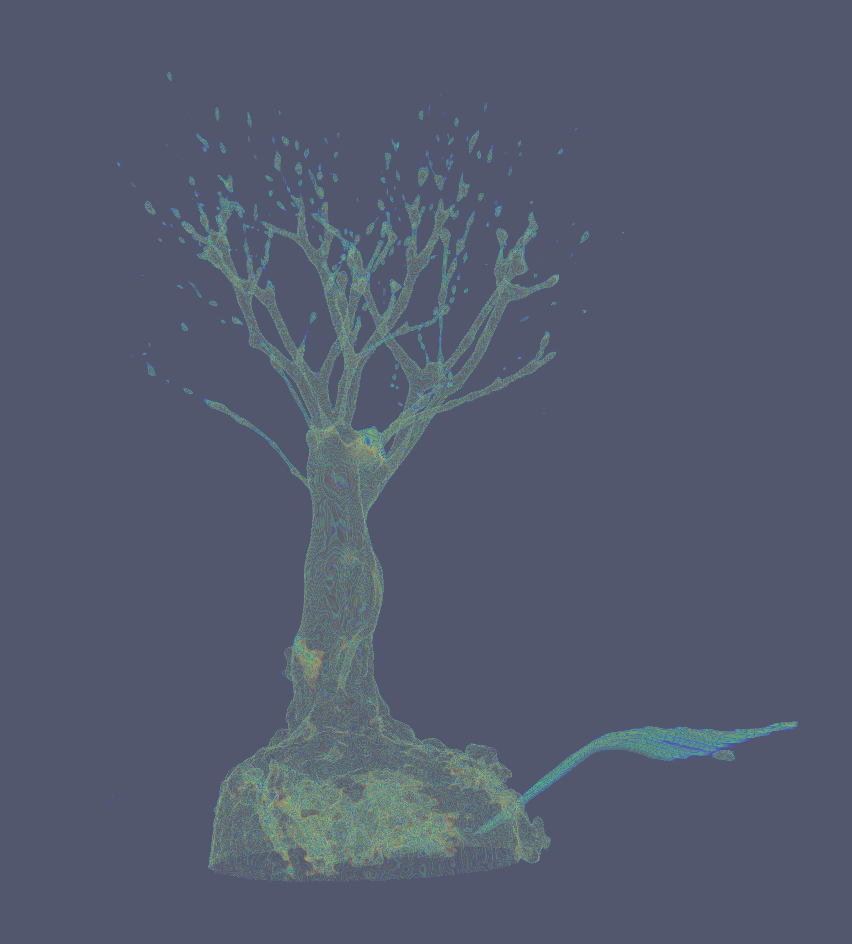
\includegraphics[width=10cm]{Tree2.png}
	\item[Tool:]
	Paraview
	\item[Visual Mappings:]
	\begin{itemize}
		\tightlist
		\item[ ]
	\end{itemize}
	\begin{itemize}
		\tightlist
		\item
		\textbf{mapping 1}: Colour mapping is set to LAB.
	\end{itemize}
	
	\begin{itemize}
		\tightlist
		\item
		\textbf{mapping 2}: Answer
	\end{itemize}
	\item[Data Conversion:] Data scalar type unsigned char was used. Along with data extent: 0 - 511, 0 - 511, 0 - 181. Repersentaion is volume.
	\item[Unique Observation:]
	At data point 76.894 is where the internal part of the tree trunk disappears. While at data point 54.696, this is where the leaves will start to dissapear from the visualisation.

\end{description}